% Drawing 154/08-28 -- folder 154, batch 08, archive page 156 (PDF page 157).
% Transcription: au-dessus de $(D_0, -\beta^{*}, \omega^{*})$, un petit dessin en couleur : deux droites orange qui se croisent ; une droite vert clair en tirets passe par le croisement, une droite verte pleine passe au-dessus (le triangle entre les deux hachuré au crayon) ; à droite, une flèche verte transverse vers le bas et une flèche verte vers la droite sous les tirets
% Kind: orange crossing with dashed green line through it, solid green line above, hatched triangle; arrows down and right. Method 2 (schematic redraw from the facsimile). Status: ok.
% Notes: Small drawing above the triple (D_0, -beta*, omega*). Two orange lines crossing; a dashed light green line through the crossing; a solid green line above it, the small triangle between that line and the crossing hatched in pencil; to the right a transverse green arrow pointing down across the dashes and a green arrow to the right below them. The dashes lie about 0.2 mm below the fitted crossing on the scan and are drawn through it. 2 orange strokes, 1 crossing, 8 dashes, 2 arrows; no letters. Read from the 400 dpi colour scan; each pair of orange strokes fitted to the ink and drawn through its computed crossing, the triangles bounded by the computed intersections with the green line; the redraw was overlaid on the scan and agrees to within a stroke's width. The felt strokes are drawn straight (slight curvature of a few strokes not reproduced). Redrawn 2026-11-12 (issue 128): to check again.
% Coordinates: 1 unit = 1 mm = 1/100 of the crop width, same scale on both axes (bbox in page fractions: [0.41, 0.187, 0.499, 0.23]).
% Redrawn by Claude (claude-fable-5-2), issue #128, 2026-11-12; not checked by a human; not compiled (no TeX in the session).
% Rights: reproduces part of the work -- behind RENDER_TRANSCRIPTS, never published by itself.
\documentclass[tikz,border=3pt]{standalone}
\usepackage{amsmath,amssymb}
\usetikzlibrary{patterns,arrows.meta}
\tikzset{Or/.style={orange!90!black}, Lg/.style={green!60!black!70}, Br/.style={brown!80!black}, pencil/.style={black!55}, mpt/.style={circle,draw,inner sep=1.3pt}, pt/.style={circle,fill,inner sep=0.9pt}}
\colorlet{Or}{orange!90!black}\colorlet{Lg}{green!60!black!70}\colorlet{Br}{brown!80!black}
\begin{document}
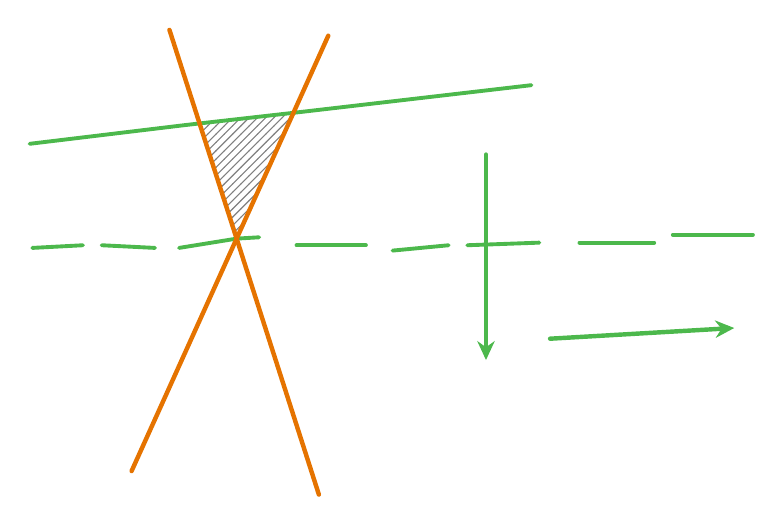
\begin{tikzpicture}[x=1mm,y=1mm,line cap=round,line join=round,font=\scriptsize]
\path[pattern=north east lines,pattern color=black!50] (30.02,-31.02) -- (25.31,-16.39) -- (37.24,-15.04) -- cycle;
\draw[Lg,line width=1.4pt] (3.73,-18.98) -- (23.39,-16.61) -- (38.31,-14.92) -- (67.46,-11.53);
\draw[Lg,line width=1.4pt] (4.07,-32.2) -- (10.51,-31.86);
\draw[Lg,line width=1.4pt] (12.88,-31.86) -- (19.66,-32.2);
\draw[Lg,line width=1.4pt] (22.71,-32.2) -- (30.02,-31.02) -- (32.88,-30.85);
\draw[Lg,line width=1.4pt] (37.63,-31.86) -- (46.44,-31.86);
\draw[Lg,line width=1.4pt] (49.83,-32.54) -- (56.95,-31.86);
\draw[Lg,line width=1.4pt] (59.32,-31.86) -- (68.47,-31.53);
\draw[Lg,line width=1.4pt] (73.56,-31.53) -- (83.05,-31.53);
\draw[Lg,line width=1.4pt] (85.42,-30.51) -- (95.59,-30.51);
\draw[Or,line width=1.6pt] (21.49,-4.51) -- (30.02,-31.02) -- (40.47,-63.53);
\draw[Or,line width=1.6pt] (41.66,-5.25) -- (30.02,-31.02) -- (16.68,-60.54);
\draw[Lg,line width=1.6pt,-{Stealth[length=2.4mm,width=2.2mm]}] (61.69,-20.34) -- (61.69,-46.44);
\draw[Lg,line width=1.6pt,-{Stealth[length=2.4mm,width=2.2mm]}] (69.83,-43.73) -- (93.22,-42.37);
\end{tikzpicture}
\end{document}
